\documentclass[a4paper]{article}


%page setting
\usepackage[left=25mm, right=25mm, top=25mm, bottom=25mm]{geometry}

%pakages
%\usepackage[colorlinks=true]{hyperref}
\usepackage{hyperref}
\usepackage{url}
\usepackage{graphicx}
\usepackage{float}
\usepackage{amsfonts}
\usepackage{amsmath}
\usepackage{amssymb}
%\usepackage{booktabs}
\usepackage{enumerate}
\usepackage{fancyhdr} %footer-header
%------underline setting--------
\usepackage{ulem}

%--------Table-related commands------
\usepackage{array} %To automatically break longer lines of text within cells, define fixed-width columns
\usepackage[table,xcdraw]{xcolor}

%\usepackage{multirow}
\usepackage{tabularx} % length of table
\usepackage{caption} %space btw caption and table

\usepackage{booktabs}
% produce heavier lines as table frame (\toprule, \bottomrule) and lighter lines within a table (\midrule).

%link: https://texblog.org/2017/02/06/proper-tables-with-latex/
\newcolumntype{V}{>{\bf\centering\arraybackslash} m{0.2\linewidth} } %Repeat column type
%------------------
\usepackage{stackengine}

%--------------Tikz-------------------------------
\usepackage{import}
\usepackage{tikz}
\usepackage{tikz-3dplot}
\usepackage{subfigure}
%-------------------------
%\usepackage[nottoc, notlot, notlof]{tocbibind}

%\usepackage{cite}
%\usepackage{natbib} % 
%\usepackage[numbers,sort&compress]{natbib} % sort of citation
\usepackage{pdfpages}

\usepackage{biblatex}
\addbibresource{citation.bib}



%\renewcommand{\baselinestretch}{1.5}
\pagestyle{fancy}
\fancyhead{}
%\fancyfoot{}
\renewcommand{\headrulewidth}{0pt}
\renewcommand{\footrulewidth}{1pt}

%------underline setting--------
\renewcommand{\ULdepth}{1.8pt}

%%==============================
%%
%%==============================
\begin{document}



\begin{titlepage}
\begin{center}
\vspace{1cm}
\large{\textbf{DEPARTMENT OF MECHANICAL ENGINEERING}}\\
%\LARGE{\textbf{CURTIN UNIVERSITY}}
\begin{figure}[h]

\includegraphics[width=\textwidth]{Curtinlogo}
\end{figure}

%\line(1,0){400}\\
\hfill\break
\hfill\break
\Large{\textbf{Milestone II for Ph.D. Program}}\\[1mm]
\vfill
%\line(1,0){}\\[1mm]
\huge{\textbf{Discrete Path Planning For Platonic Solids}}\\[1mm]
%\large{\textbf{- This is a Sample Title -}}\\[1mm]
%\line(1,0){400}\\[1mm]
\vfill

By NGOC TAM LAM\\
19107262\\
\vfill

Dr. Lei Cui (Supervisor)\\
Prof. Ian Howard (Co-Supervisor)\\
AProf. Jonathan Paxman (Chairperson)\\
\vfill
\today\\
\end{center}
\end{titlepage}

%-------------------------
\tableofcontents
\thispagestyle{empty}
\clearpage

\setcounter{page}{1}

%%==============================
%%			CONTENT
%%==============================

%
%
\noindent\section{ABSTRACT}
%\textcolor{red}{250 words or less, concise summary of research conducted, results obtained, and conclusion reached}
In the modern manufacturing industry, path planning in industrial robot applications is an important step to find the shortest direction of achieving a task. Among the path planning algorithms, graph search or exploration methods has been applied for robotic in a high-dimensional space. 
In the geometrical scenarios, the problem of path planning of polyhedra with rolling contact is considered. However, their rolling behaviour with returning to the initial configuration in different orientation has remained unexplored. To tackle the problem, this study proposes a path planning method for regular platonic solids through rolling contract on a plane based on an improved tree search algorithm.
The results reveal that the proposed path planning method can enhance the efficiency of the planning for regular convex polyhedra.
Consequently, Matlab simulations are conducted in order to demonstrate the proposed algorithm in terms of finding the shortest path of rolling the regular platonic solids in a discrete environment.

%\textcolor{blue}{\uline{Background}: Place the question addressed in a broad context and highlight the purpose of the study.}\\
%
%
%\textcolor{blue}{\noindent\uline{Aim}: }\\
%
%\textcolor{blue}{\noindent\uline{Approach}: Methods: Describe briefly the main methods or treatments applied;}\\
%
%\textcolor{blue}{\noindent\uline{Significance}:Results: Summarize the article’s main findings;}\\ 
%
%\textcolor{blue}{\noindent\uline{Conclusion}: Indicate the main conclusions or interpretations. The abstract should be an objective representation of the article, it must not contain results which are not presented and substantiated in the main text and should not exaggerate the main conclusions.}
%
%Examples: from "2018 Path Planning of Industrial Robot - RRT"
%
%With the development of modern manufacturing industry,the application scenarios of industrial robot are becoming more and more complex. Manual programming of industrial robot requires a great deal of effort and time. \textbf{Therefore}, an autonomous path planning is an important development direction of industrial robot. 
%
%Among the path planning methods, the rapidly-exploring random tree (RRT) algorithm based on random sampling has been widely applied for a high-dimensional robotic manipulator because of its probability completeness and outstanding expansion. \textbf{However}, especially in the complex scenario, the existing RRT planning algorithms still have a low planning efficiency and some are easily fall into a local minimum. 
%
%\textbf{To tackle these problems}, this paper proposes an autonomous path planning method for the robotic manipulator based on an improved RRT algorithm. The method introduces regression mechanism to prevent over-searching configuration space. 
%\textbf{In addition}, it adopts an adaptive expansion mechanism to continuously improve reachable spatial information by refining the boundary nodes in joint space, avoiding repeatedly searching for extended nodes. 
%\textbf{Furthermore}, it avoids the unnecessary iteration of the robotic manipulator forward kinematics solution and its time-consuming collision detection in Cartesian space. The method can rapidly plan a path to a target point and can be accelerated out of a local minimum area to improve path planning efficiency. 
%
%The improved RRT algorithm proposed in this paper is simulated in a complex environment. The results reveal that the proposed algorithm can significantly improve the success rate and efficiency of the planning without losing other performance.\\






%\section{OBJECTIVES}

\noindent The aim of this research is to generate a new mathematical model of rolling-based robotic in-hand manipulation in discrete space.  In addition, rolling contact in the multi-fingered robot hand is further considered. The specific objectives for this research project are as followed by steps below:
\begin{enumerate}[(i)]
  \item Discretized rolling contact model: An initial task of the study is to develop the geometrical framework in discrete space to form differential geometry of the rolling contact between two models (an object and robot fingers) in terms of moving frame, curvature, torsion, and the Lie-group theory.
   
  \item Discrete path planning for polyhedrons: The task is required to examine whether the path exists under solving the motion planning problems and then to generate these paths. The discrete path planning will be investigated from regular polyhedrons to general polyhedron. Discrete search algorithms are approached to locate a grid resolution and the discrete contact will be analyzed for the path planning process. 
  
  %\item Discrete  path generation: Discrete planning will be investigated by state-space models involving the distinct situation (state) and the set of possible states (space). The connection from an initial configuration to goal configuration in discrete space can generate the discrete path under rolling contact between an object and multifingered robot hands.  
  
  %When the path exists, how can I generate/find the path?
  
  \item Optimal path planning: Because path planning between the object and multifingered robot hands faces with the high dimensional environment, the optimal path planning should be considered. I also propose the analysis technique to improve both cost and capacity of the discrete path planning under rolling contact condition in terms of discrete differential geometry. 
  
  %I can find the path, how can I know whether the path is optimal or not?
  
  \item Experimental validation for dexterous robot in-hand manipulation: At the last stage of the study, Matlab and Robot Operating System (ROS) will be used to test the system in simulated environment and then ABB robot arm is integrated to BarrettHand to run the system as a physical robot.
  
\end{enumerate}



%$=>$ build up a discrete framework to formulate and solve the motion planning problems.
%\section{BACKGROUND}
\uline{Introduction.} 
Rolling contact has been studied considerably in the literature. Rolling contact is described different types by point contact \cite{Cai86_PlanarMotion_PointContact, Cai87_SpatialMotion_PointContact} , line contact \cite{Cai88_SpatialMotion_LineContact}, and surface contact \cite{Borisov08_ChaplypinBall_FixSphere}. Many researches in the field of geometry \cite{Montana88_Kinematics_Contact_Grasp}, controllability \cite{Marigo00_RollingBodies_Controllability}, motion planning \cite{Z.Li91_NonholonomicMotionPlanning} or robot manipulation \cite{Murray-Li_EbookRobotic_Manipulation} demonstrated that rolling contact in terms of robot manipulation, especially in multifingered robot hands, has played an important role in recent decades. However such simple end-effector through multifingered robot hands can relocate only a few objects and the dexterity of robotic in-hand manipulation still need to study.\\

%Rolling manifolds[]\\

\noindent\uline{Research focus.}
The purpose of this research firstly focuses on the continuous and discrete path planning generation methods and then employs discrete rolling contact theory in in-hand manipulation and enhances robot hands working dexterously in discrete space as the motivation of this study. The optimal path planning is also considered to eliminate the cost of the process of path generation. Therefore, developing the discrete contact theory in terms of differential geometry is significantly considered in this research. Experimental validation is the final step to test the whole system including physical robot.

\subsection{Rolling Contact}
%-------------------------------------------------------
%				Classical Nonholonomic system
%-------------------------------------------------------
%\uline{Classical nonholonomic system}.

%-------------------------------------------------------
%				Rolling contact in continuous space
%-------------------------------------------------------
\noindent\uline{Rolling contact in continuous space.} 
Rolling contact through ball-plate and rolling sphere problems of nonholonomic systems has been intensively investigated in the past by many researchers \cite{Robert00_BallRolling_OnSphere, Borisov08_ChaplypinBall_FixSphere, Borisov08_Dynamics_NonHolonomic, Borisov08_ExplicitIntegration_NonHolonomic}. Later than, Hartmann \cite{Hartmann00_Blending_ContactCurves} applied a numerical blending method to develop the classical rolling ball method in terms of constant and variable radius through analyzing the Voronoi surface, Bezier surface and G$^2$-blending surface. Especially, the rolling sphere model by Brockett \cite{Brockett93_NonholonomicKinematic} has the asymptotic stability problem of the five dimensional nonholonomic systems that can be transformed into a chained form system. A specific  geometric formulation in terms of curvature of rolling motion between a sphere and two arbitrarily shape fingers was derived by Montana \cite{Montana88_Kinematics_Contact_Grasp}, of which this paper refers to the special case - a rolling sphere and a plate. This rolling contact condition is formulated as a contact equation via the differential geometry concepts - a well-known nonholonomic constraint.\\

%-------------------------------------------------------
%				Kinematic of rolling contact
%-------------------------------------------------------

\noindent\uline{Kinematic of rolling contact}.
%\textcolor{red}{•Reduce the length of the discussion on modelling the kinematics of rolling motion}\\ 
%A simple definition of kinematic chain is a coordinate transformation that demonstrates the relationship between the position and orientation of an object and the fingers \cite{Montana95_kinematic-multifingered}. 
A part of rolling contact is considered in terms of the kinematics which are essentially analyzed from dynamics 
\cite{Sarkar97_DynamicControl_3D_RC, Arimoto03_DynamicForceTorque_MeanRC, Svinin13_Dynamic_MP_SphereRollingRobot}, controllability \cite{Yun92_Control_RC, Zribi99_Control_RC, Marigo00_Control_RollingBody, Nakashima05_ControlGraspManipulation_RC} and motion planning 
\cite{Cai86_PlanarMotion_PointContact, Z.Li89_MotionPlanning_Dex.Manipulation, Chelouah01_MotionPlanning_RollingSurfaces, Svinin08_MotionPlanning_RollingSphere}. 
The majority of study in multifingered robot hands has been involved in differential equations based on kinematic. Cai and Roth \cite{Cai86_PlanarMotion_PointContact} used Taylor series expansion to derive the first and second order of kinematics of sliding-rolling. 
%Salisbury and Craig \cite{Salisbury-Roth83_Kinematic_Force_ArticulatedMEHand} explicitly stated that the contact degree of freedom are virtual joint. These authors also developed the analysis of the contacts between bodies which have the constraints within the effects of friction while \cite{Z.Li89_UnifiedControl, Murray90_GraspingManipulation} discussed the constraints on the fingertips with friction can be arbitrary kinematics constraints. 
Okamura \cite{Okamura_2000_Overview_DM} developed Jacobian relationships in developing dexterous manipulation kinematics. However, the system may be over-constrained or under-constrained that hardly maintains the rolling contact property. 
Another series of study about kinematics in terms of rolling contact was conducted by Lei 
\cite{Lei10_Geometric.Kinematics_PointContact, Lei12_Polynomial_Inverse.Kinematics, Lei12_ReciprocityBased_SVD_Inverse.Kinematics,
Lei15_sliding.rolling.loci_kinematics,
Lei15_PolynomialFormulation_InverseKinematics, 
Lei17_In-Hand_Forward.Inverse.Kinematics, Lei18_Rolling.Contact_Kinematics_Multifinger}. The author applied the theory of Darboux moving frames method in differential geometry to demonstrate the contact equation between an object and multifingered robot hands and generate the forward and inverse kinematics of in-hand manipulation.\\

%-------------------------------------------------------
%				Cantan's moving frame
%-------------------------------------------------------

\noindent\uline{Contact theory via Cartan's moving frame method}. Cartan's moving frame method is essential approach for geometric objects in contact kinematics \cite{H.Cartan96,E.Cartan02}. The method  was widely applied in the computation of symmetry groups, partial differential equations \cite{Mansfield01_AlgorithmSymmetric_Diff, Morozov02_MovingFrame}, geometrical curves and surfaces \cite{Beffa03_relative_Absolute_DiffInvariant, Beffa06_PoissonGeometry_DiffInvariant} or finite dimensional transformation group from Lie algebras \cite{Boyko06_LieAlgebra, Boyko07_LieAlgebra}; however, there has been little attention to the robotic field. One of the remarkable studies from Lei \cite{Lei10_Darboux-Frame} is to explore differential geometries in terms of curvatures of shapes through the spin motion to establish the contact theory. \\
%\cite{Lei09_coordinate-free_instantaneous_kinematics, Lei10_Geometric.Kinematics_PointContact,  Lei15_sliding.rolling.loci_kinematics, Lei15_PolynomialFormulation_InverseKinematics}

 

%-------------------------------------------------------
%				Rolling contact in discrete space
%-------------------------------------------------------
\subsection{Motion Planning and Path Planning}
\uline{Introduction.} 
Motion planning is the most important task of robotics research \cite*{Sudsang_2000_Grasping_In-hand_manipulation},\cite*{Pajarinen_2017_R.Manipulation_POMDP} in static and dynamic environment as an emerging area for a long time. The path planning strategy for robotic research can be categorized into traditional methods and discrete approach or also divided into two folds as the local path planning and the global path planning strategy. However, most of the previous studies focus on mobile robots, unmanned aerial vehicle (UAV) or autonomous sef-driving car while only few research has been implemented on the rolling contact of robotic in-hand manipulation. 

\subsubsection{Traditional Motion Planning}
%The topic on motion planning can be divided into three main categories as follows. 
Reaching the final configuration and reducing the cost of path generation within the minimum distance and time are the most important tasks of robotic motion planning. There are various approaches proposed/implemented by many researchers that are highlighted below.\\

\noindent\uline{Roadmap approach.} 
Roadmap is one of the classical techniques has been focused on the precise motion planning where the configuration-free space is withdrawn into the system of 1D lines. The connectivities of the free space \textit{F} are captured by a network of 1D curves such as Voronoi diagrams, roadmap \cite{Canny88_PhDThesis}, Star-shaped roadmap (a deterministic sampling approach) \cite{Varadhan05_StarshapedRM} and criticality based method \cite{Latombe99_JourneyRobotics}. There are some drawbacks on these methods including the computation of free space and less practical algorithms for computing these methods of large environment.\\

%-------------------------------------------------------
%				
%-------------------------------------------------------
\noindent\uline{Classical cell decomposition approach.}
Another classical method of motion planning is called cell decomposition which is divided into full cell, empty cell and mixed cell \cite{Latombe91_FastPlaner}. The advantages of this method is to compute the planning process incrementally which represent a sequence of cell connecting. The borders between all the cells, which are assigned as the function of the environment, may represent the favourable circumstances of the cell decomposition method. However, the method is still not to compute the free space precisely that can be approached as a dual to the roadmap method.\\

%-------------------------------------------------------
%				
%-------------------------------------------------------
\noindent\uline{Potential field category.} 
It is quite different from two previous approaches that the connectivity graph in potential field method is not required to pre-compute in the process of path generation. In stead, searching of a path is guided by a heuristics and constructed by an artificial potential function which is represented the sum of potentials (achieving the goal configuration and avoiding the obstacles) \cite{Khatib85_ObstacleAvoidance}. The potential field is distinct across to avoid obstacles in each time-step. The advantage of this method is that various its application can be applied for the movement of nonholonomic mobile robots or human-robot interaction. \\


%-------------------------------------------------------
%				Non-holonomic motion planning
%-------------------------------------------------------

\noindent\uline{Non-holonomic motion planning.} Non-holonomic motion planning has received much attention in the past. The simply definition of non-holonomic robot motion planning is the movement of the robot from an initial configuration to a desired configuration  \cite{Z.Li89_MotionPlanning_Nonholonomic, Z.Li91_NonholonomicMotionPlanning, Murray93_NonholonomicMP}. 
The motion planning of the object to acquire a desired configuration and the grasp planning in terms of contact force optimization are two main categories of dexterous motion planning \cite{Okamura_2000_Overview_DM}. 
Specific motion planning of rolling surfaces in terms of chained-form has been introduced by several authors such as Brockett \cite{Brockett82_ControlTheory_RiemannianGeo} who introduced sinusoidal inputs then the method was developed in more detail by Murray et. al \cite{Murray-Li_EbookRobotic_Manipulation}. 
However, a challenge from these studies is that the triangularized form of the system equation could not transform into chained-form.\\

%However, the article \cite{Bicchi95_Dex.Manipulation_Rolling} could not transform the triangularized form of the system equation into chained-form while Monaco \cite{Monaco92_MP_DigitalControl} investigated non-holonomic chained systems through the two constant inputs where they achieved the interactive planning schemes.\\

%\noindent\uline{Optimal motion planning.} using Reinforcement learning, and clearance based path optimization for MP: \cite{Gomez11_RL_MotionPlanning, Geraerts04_PathOptimization_MP}\\ 
%\cite{Khalidi18_TStar} T*: A heuristic search based algorithm for motion planning with temporal goals $=>$ Combine with Temnporal Goal to optimize the graph search. 

\noindent\uline{Path planning for two general objects.}
Rolling contact between two objects under nonholonomic constraint is usually a difficult task to work with. In terms of path planning under rolling constraint, the study \cite{Z.Li90_MotionRigidBody_RC} used the Gauss-Bonnet theorem in differential geometry to generate a path for the contact between two unit balls. The approach of path planning was considered through a nonlinear control problem in terms of the control vector fields and the control inputs. The study applied the geometric data such as curvature forms, metric tensors and connection forms in order to find an admissible path between two contact configuration under nonholonomic rolling constraints.\\

%\textcolor{red}{•Add a brief review of path planning for two general objects under nonholonomic constraints}\\
%-------------------------------------------------------
%				Discrete Planning
%-------------------------------------------------------
\subsubsection{Path planning in discrete space}
\noindent\uline{From continuous to discrete.} Path planning of robots in complex environments has received quite a lot of attention in the past while only a few studies have focused on discrete space. Interestingly, combining computation frameworks and the discrete algorithms was considered in recent studies to capture the complex environment \cite*{Belta_2005_Discrete_MP}. 
This method is combined with the continuous path planning \cite{Mitchell03_ContinuousPathPlanning} that can generate or model the kinematics, control laws and a path of the robots. Therefore, the computational framework for automatic path planning for robots in unknown environment in discrete space also needs to be considered.\\

%-------------------------------------------------------
%There are few studies on discrete space.\\ \textit{From Belta \citep*{Belta_2005_Discrete_MP}. There has been interest recently in creating computational frameworks combining the discrete algorithms capturing the complexity of the environment with the continuous approaches modeling the kinematics or dynamics of the robots. 



\noindent\uline{Discrete path planning.} Planning techniques are categorized into different aspects. The basic idea of discrete path planning in the most cases is that state-space models will be used to demonstrate the distinct situation in which the task of a planning algorithm solves the sequence actions transforming from a initial state to other states \cite{LaValle06_PlanningAlgorithm}.
For example, Thomas \cite*{Thomas_2003_Trajectory} applied Delaunay triangulations to discretize the environment, and cubic spline representations are proposed to meet robot kinematic constraints.
Considering the continuous curvature on smooth curves has been integrated within the probabilistic approaches in order to compute the piecewise smooth paths for a car-like vehicle as a four-dimensional system \cite*{Lamiraux_2001_Smooth_MP}. Whereas, dealing with nonholonomic constraints, a sampling-based road map technique was proposed in \cite*{Cheng_2001_RRT_trajectory}. Based on decomposing space into cells \cite*{Conner_2003_Potential_Func}, a potential field without local minima was assigned with polygonal partitions of planar environments to solve the Laplace's equation problems in each cell exist.\\



%-------------------------------------------------------
\noindent\uline{Probability cell decomposition.} The simple idea of this method is to determine a path between an initial configuration and the goal configuration in the way of dividing the free space into cells. There are two terms of the method including an approximation cell decomposition and an exact cell decomposition\cite{Lingelbach04_PP_ProbabilisticCellDecomposition, Rosell05_PP_Harmonic_ProbabilisticCellDecomposition}. 
The former methodology refers to a decomposition in which the cells is bounded approximation by the free space that can allow the robot finalizes the motion planning tasks with complex geometries to achieve connectivity paths.
Exact cell decomposition has the first step to decompose the free space into trapezoidal triangular cells then nodes which represent cells in the connectivity graph are adjacent in the configuration space.
However, there are intensive time and memory on the computation of decompositions and limited volume of the configuration space, which rise exponentially with the DOFs of system.\\ 



%-------------------------------------------------------
\noindent\uline{Randomized potential field algorithm.} Precomputation of a connectivity graph of the global path-planning which contains the guide for grid search in the configuration space is the high cost for computation system. Using the properties of potential function \cite{Barraquand91_MP_DisctributedRepresenation}
can generate no systematic way to escape the minima at the goal configuration. The technique in the first step is the best-first search which does not require to reach a local minimum of the potential function in hight-dimensional configuration spaces. Then the search algorithm which proceeds along the negated gradient of the potential function until the goal configuration is achieved. The most powerful of this method is to discretize the configuration space and the work space into a hierarchical bitmap grid that can be applied for many DOFs of robots.\\

%-------------------------------------------------------
\noindent\uline{Rapidly-exploring Random Trees (RRTs) and RRT-Connect.} RRTs is a randomized data structure technique to solve a planning problem \cite{Lavalle98rapidly_exploringrandom}.
The method does not require any connections of nearby configurations. It can be applied for path planning problems in terms of the nonholonomic constraints and high degree of freedom. The method still remains on the trajectory optimization problems. Another study in \cite{Kuffner00_RRTConnect} improved the RRTs method called RRT-Connect technique which combines the RRTs and a greedy heuristic to speed up the exploration of configuration (state) space and the connection from an initial configuration to other goals. However, these challenging issues still remain in terms of computational geometry such as the artificial bias which can be given from searching nearest-neighbour to the convergence rate.\\
%Following \citep*{Cheng_2001_RRT_trajectory} page3\\




%-------------------------------------------------------
\noindent\uline{Probabilistic Roadmap Planer-PRM.}
The PRM technique has been successful for path planning problems, which was implemented in different sites \cite{Amato96_PRM_PathPlanning, Kavraki95_Thesis_RandomNetworks_FastPlanning, Overmars92_RandomApproach_MP}. 
The PRM computation consists of two phases: the preprocessing phase and the query phase. Repeating the generating random free configuration space can generate a probabilistic roadmap in the preprocessing phase. The nodes of the graph and the paths are computed through local planner that can create the graph edges. In the query phase, there is starting by connection between the initial and the goal configuration by a Dijkstra's shortest path query \cite{Geraerts04_Comprative_PRM}. Finding complete edges from connecting nodes in the roadmap to generate a graph search is the feasible path for the planning problem. Nevertheless, Probabilistic Roadmap Planner method should be optimized due to some reasons such as the low quality of searching process - the graph is a tree, not cycle graphs and involving straight-line motion which generates the first order discontinuities at the nodes. \\



%---======---=-=-=-=-=-=-=-=-=-=-=-=-=-=-=-=-=-=-=-

%-------------------------------------------------------
\noindent\uline{Heuristic search method.} 
The fundamental robotic path planning problem is to represent the environment as a graph involving the set of possible robot location and a set of edges that can generate the paths. The popular method for determining the least-cost paths is A* as Heuristic based search algorithm in  \cite{Hart68_HeuristicDetermination,
Nilsson82_Principles_AI, 
Rankin_1996_A_star_Search}.
The search algorithm must expand the fewest possible nodes in order to make searching for an admissible path. Then the evaluation of available nodes is needed to determine the next efficient nodes.
The initial search approached by A* takes two steps to generate an optimal path in which receiving information from one of the initial cells in free space and replanning from scratch when the environment has changed to expand a new cell.
However, the A* computation process needs high configuration processors to successfully reach various nodes. In the real world scenarios, the search operating sometimes may be performed with inaccurate planning graphs.\\
%From \cite{Ferguson05_HeuristicPathPlanning, Hoang15_HeuristicPathPlanning}.\\

%-------------------------------------------------------
\noindent\uline{Dynamic programming.}
Dynamic programming (DP) is a technique of robot path planning problem solving to calculate the distance of the goal configuration from all the initial configuration in the grid map \cite{Bellman57_DynamicProgramming}. 
The environment in most robot path planning issues is implemented by a topologically organized map where the connections between each grid points and their neighbouring grid points are built. The distances at every iteration are updated to constitute the neighbour cells when the environment is discretized into a grid of points. 
As proof in \cite{Bellman57_DynamicProgramming}, the DP method can provide a simple approximation to optimize the trajectory solution that does not suffer from the curse of dimensionality. 
A criticism of DP that has precluded the practical implementation in path planning problems is somewhat more difficult for executing the DP algorithm due to time consuming \cite{Kala12_RobotPP_DynamicPlanning}.
The efficient cost is the property of the DP method by sub-dividing the complex problems into sub-problems and converging various steps of solving sub-problems. However, the expense of the DP algorithm is not as overwhelming nowadays thanks to the faster and stronger computer and the parallel-processing computer which can efficiently execute the expanding nodes.  \\

%-------------------------------------------------------
\noindent\uline{Genetic algorithm technique.} The genetic algorithm was initially proposed by Holland \cite{Holland75_GAMethod} as a non-conventional method. The GAs method has been applied for a wide assortment of problems such as natural genetic operators-reproduction, mutation, and crossover. GAs benefits the great solutions for upgrade problems to find an optimal path of the mobile robots from an initial configuration to the goal configuration in a grid environment. The GA technique currently is used to find the shortest path in terms of less number of generations in different environments such as indoor, moderate or complex scattered environment. However, the GAs tend to find a feasible path without considering the distribution and location of obstacles in the unknown environment.\\

%-------------------------------------------------------
%\noindent\uline{Temporal-difference learning.} From Sutton Bartol.\\


%-------------------------------------------------------
%\noindent\uline{Other general search methods.} Breadth first, Depth first, Dijkstra's algorithm, Backward search, Bidirectional search. Monte Carlo methods. Temporal-difference learning.\\


%-------------------------------------------------------
%				Optimal path Planning
%-------------------------------------------------------
\noindent\uline{Optimal path planning.}
In order to optimal paths which are generated from various path planning techniques, an introduction of a new method based on the randomization and the dynamic programming was proposed in \cite{Sallaberger95_OptimalPP_DP_Randomization}.
The method normally is used to optimize paths for mobile robots and articulated robot manipulation. Using only the dynamic programming can lead to cost of calculating the path segments from one cell to other grid cells because of the large size of the search space, especially for curse dimensional issues. To overcome this problem, the use of randomization in the discretized grid within the dynamic programming may reduce the cost path. Considering the orthogonal neighbour relations that are connections between a node and orthogonal one another can decrease the computations. 
Another study in \cite{Devarus16_Optimal_PathPlanning} called Sampling-based algorithm based on the Rapidly-exploring Random Tree (RRT) algorithm by combining the Transition-based RRT (T-RRT) and RRT* can solve complex high-dimensional path planning problems and converge faster to the optimal path. \\ 

%\textcolor{red}{•If optimal planning is discussed, ensure you are specific about in what sense the solution is optimal. In some cases, optimality is not required, only a satisfactory or satisficing solution in the sense of a cost function being below some bound. In such cases, sampling-based solutions (such as RRT) are appropriate.}\\

%==============================================================
\subsection{Discrete Polyhedron Path Planning}
\noindent\uline{Introduction.} Manipulation of industrial parts mostly based on the robotics problems in the different domains like car assembly manipulation. The multifingered robot hands has been used to manipulate the object flexibility. However, the application of this term may applied for regrasping \cite{tournassoud1987regrasping, goldberg1993feeding}, pushing and tilting objects \cite{erdmann1993mechanical, peshkin1988planning} with integrating into the end-effectors in industrial robots. In this study, I will focus on the geometry contact from rolling contact manipulation in the nonholonomic behaviour.\\


%\textcolor{red}{•Include a section which describes how a discretised model will be produced such that the discrete planning algorithms described can be applied. How is this discrete model to be obtained from the continuous-time models discussed?}\\

\noindent\uline{Discretised continuous-time models.}
While the classical differential geometry focus on the smooth geometric shapes, discrete differential geometry investigates geometric shapes with a finite number of elements such as polyhedra \cite{Discrete_ComputationalBook}. In terms of rolling contact in discrete space, the models will be discretized into discrete surfaces or quadrilateral faces which called discrete parametrized surfaces. The study of rolling contact between two models will be focused on the contacts of discrete surfaces, with an emphasis on the geometrical structures of discrete systems.   \\



\noindent\uline{Polyhedron manipulation.}
There are various types of a polyhedron moving on a plane such as sliding on a face, rolling through the edges or pivoting about the vertex. The planning motions of rolling polyhedra parts through the edges was clearly represented in \cite{Marigo97_PolyhedraManipulation_rolling}. The paper showed the rotations of a polyhedron based on edges into a fixed plane under considering a polynomial time for planning tasks. Experimental work is implemented in the article to represent manipulation of rolling polyhedron on a plane.
The set of configurations has different structures with different polyhedra that can be reached by rolling their edges. An example from the article showed that a unit cube will reach the next position by rolling $\pi/2$ along the edges on a square mesh. However, it is quite different from a truncated pyramid that one wishes can be represented for the achievement of the arbitrary configuration.\\

\noindent\uline{A simple case of disk rolling on a plane.}
The paper \cite{Erdmann91_polyhedronRolling_on_table} focused on the finite friction contact between the faces of polyhedron and the table regarding to disk rolling on a tiltable table. In the simple experiment was conducted in the paper, a polyhedron surface was discretized in a list of surfaces. The author used Markov transition which corresponds to the face-to-face contact between polyhedron surfaces and the table in order to perform the rolling contact theory under considering the infinite friction and ignoring the inertial and impact forces. The orientation is described through tilting of the table that represents the two degrees of motion freedom. A $\theta$ title angle of the table tilting from the horizontal axis ranging from $0$ to $\pi/2$ assumed nearly instantaneously. This paper solved the simple problems of orienting parts on a plane through combination of probabilistic and geometrical analyses in terms of nonholonomic system.\\


\noindent\uline{Polyhedra-based rolling planning motion.}
Marigo \cite{Marigo2000_Polyhedral} proposed the path planning for polyhedron in the case of octahedron with 8 faces rolling and translating on a plane.
For the octahedron rolling algorithm, a list of faces containing the vertices and edges stored parts of polyhedron. The defect angles are also computed for each of vertices. The algorithm was given a polyhedron with a set of geometrical parameters and a desired final configuration. The steps of planning include translating and rolling until achieving the final configuration. However, the algorithm may not satisfy with the accuracy for more general polyhedra.\\





%\noindent\uline{Dexterous polyhedron rolling} Another aspect of an object orientation was described in (Rus92) that the finger tracking with the fixed fingers was applied to manipulate the axis and angle of the object rotation. The implementation of instantaneous rotations focused on tetrahedra and for arbitrary polyhedra. In the case of tetrahedra rotation, the path planning was built by knowing the instantaneous finger motion from the given initial configuration to desired instantaneous motion of the object. \\ 



%\noindent\uline{Convex polygon avoid obstacles} Convex polygon moving and rotate in free space to avoid obstacles [6] "A subdivision algorithm in configuration space for findpath with rotation"\\ Polygon moving to avoid polygon obstacles in the environment [5]\\ Polyhedral object moving to avoid polyhedral objects in a static environment [13] \\


%==============================================================
\subsection{Robotics In-hand Manipulation}
\noindent\uline{Dexterous manipulation.} Simple definition of dexterous manipulation is to manipulate motions of an object and to move the object from an initial configuration to a desired configuration via a given trajectory \cite{Okamura_2000_Overview_DM, Bullock11_Classify_HandManipulation, Ma_2011_dexterity_DM}. The dexterous manipulation of an object using multi-fingered robot hand is one of the problems. Li et. al \cite{Z.Li89_MotionPlanning_Dex.Manipulation} proposed grasp planning algorithm in terms of stability and manipulability and the control algorithm for the coordinated manipulation by a multi-fingered hand. Bicchi et. al \cite{Bicchi95_Dex.Manipulation_Rolling, Bicchi_2000_RC_Dexterous} demonstrated the technique to achieve the dexterous manipulation via rolling contacts. 
The author used a continuous method proposed by Sussmann \cite{Sussman93_Continuous_Nonholonomic_Path} which implemented the dexterous manipulation of an object of arbitrary shape. 
Developing the technique for dexterous manipulation by integrating the theory of kinematics and nonholonomic motion planing, Han \cite{Han97_Dex.Manipulation_RC} conducted an experiment on dexterous manipulation with multifingered robotic hands with rolling contact.\\

%==============================================================
%\noindent\uline{Reinforcement learning for dexterous manipu%lation}From (RL for Dexterous Manipulation TaskBachelor thesis).\citep*{Wright_1989_dexterity} \textit{a taxonomy of different human grasps is introduced and various motion primitives are identified. Two possible primitives, for example, are acquiring an optimal grasp or turning a grasped object about one axis.}\\


%==============================================================
\noindent\uline{Tactile feedback in in-hand manipulation.} Tactile sensing in robot hands is mostly conducted as the continuous sensing to enhance the dexterity and ability of object manipulation \cite{Howard89_SurveyofRobot_TactileSensing}.
Tactile feedback plays an essential role for dexterous multifingered-robot hand manipulation tasks. With additional information from tactile sensors, the robustness and the ability to react can be improved by detecting instabilities, disturbances or slippage \cite{Bekiroglu_GraspStability_Tactile, MiaoLi_GraspAdaption_Tactile}. However, there are some tools such as the moving frame and curvatures from the geometric differential properties has not been discussed in rolling contact in in-hand manipulation.\\

%==============================================================
\noindent\uline{Manipulation by rolling contact.} Since rolling contact is nonholonomic constraint, the multifingered robot manipulation by rolling contact plays an important role in the improvement of dexterous manipulation. Generally, the manipulation by rolling contact has been considered in different view points including manipulation of objects by multifingered robot hands or consideration of contact points for nonholonomic systems. The study of a three-fingered robot hand manipulating an object has been considered by Cole et al \cite{Cole89_Kinematics_multifingered-RC} that was extended by Sarkar et al \cite{Sarkar97_DynamicControl_3D_RC} in terms of manipulating an object under the pure rolling contact. However, these studies have not been utilized and the study of the contact point has not been demonstrated enough.\\

%\noindent\uline{Control-Manipulation} Classical methods for manipulation and craft sophosticated control rules \citep*{Han_Trinkle_1998_DM_Rolling, Cherif_1999_planning, Doulgeri_2013_RC}. It works on a well known environment or for a small number of tasks.\\


%-------------------------------------------------------
%				Contact in manipulating
%-------------------------------------------------------
%\noindent\uline{Contact in manipulating.} Manipulating the objects via contacts may divide into different types such as point-contact with friction (or "hard finger”), or "soft finger”, and complete-constraint contacts (or "very-soft-finger”). Sliding and rolling conditions also are important aspects of contact modeling. The contact point moves on the contacting surfaces as they rotate with respect to each other or not which is considered as an idealized situation of contact between surfaces with infinite relative curvature.\\

















%

\section{SIGNIFICANCE}
\noindent\uline{Research gap.}
As deeply searching on the literature review, integrating tactile sensors into robot hands may improve the dexterity of robot in-hand manipulation \cite{Lei14_Teleoperation_ThumbRobotHand} \cite{Bagnell12_IntegratedSystem_AutonomousRoboticsManipulation} that may emulate human sensing.
However, there were not significant investigations into discrete differential geometry and rolling-based multifingered robotic in-hand manipulation. Specifically, discrete path planning has not been proposed for the general polyhedron in rolling contact and the cost and capacity of path planning under discrete rolling contact also need to be optimized.\\

%Besides, the important tools in differential geometry including curvature theory and Lie group theory are formed to approximate geometry attributes \cite{Lei09_Kinematic.Geometry_Circular.Surfaces, Lei09_coordinate-free_instantaneous_kinematics, Lei10_Darboux-Frame, Lei10_Geometric.Kinematics_PointContact, Lei15_PolynomialFormulation_InverseKinematics, Lei15_sliding.rolling.loci_kinematics}. 
%----------------------------------------------------------------
\noindent\uline{Research outcome.}
During the PhD program, I propose to develop a discrete contact theory based on the discrete differential geometry; then apply this tool to implement the dexterity of rolling contact into the robotic hands. 
Discrete path planning tasks will be proposed though the improvement of RRT-connect and RRT* algorithms. Then the Bellman equation will be solved for optimal path planning of the general polyhedron.
The research will apply for robot manipulation that contribute to the development of robot hands to achieve human-like capacity for in-hand manipulation. Not only the academic sector, the industrial applications are also benefited from the research. 



%\textcolor{red}{\textit{•	Include a discussion of the motivation and advantages for rolling contact for in-hand manipulation}} 
%\section{RESEARCH METHOD}
\noindent\uline{Proposed methodology.}
The research aims to propose a new discrete contact theory which will develop the capacity of tactile sensing in robot hands. To begin, the deep exploration of literature review on the theory of rolling contact in multifingered robot hands in both continuous and continuous spaces. Then, it is also important to build up a new mathematical model of the discrete rolling contact which can apply on the object manipulation by multifingered robot hands. To complete the proposed study, the process should be separated into three main steps: theoretical approach, simulated system, and experimental validation.\\

\noindent\uline{Theoretical approach.} The study mainly focuses on the rolling contact between robot hands and objects in discrete space. Firstly, it is crucial to explore the previous theory from continuous to discrete differential geometry as the tools to describe the rolling contact. It can be referenced from previous studies in 
\cite{Lei09_coordinate-free_instantaneous_kinematics, Lei10_Darboux-Frame, Lei15_PolynomialFormulation_InverseKinematics, Lei15_sliding.rolling.loci_kinematics, Lei10_PhDThesis}
which described the contact theory in terms of the moving frame, normal curvature, geodesic curvature, and geodesic torsion. In the next stage, specifically reviewing the path planning of regular and general polyhedron in discrete space is also proposed in the study. Finally, the discrete contact theory will be applied for the robotic in-hand manipulation.\\

\noindent\uline{Simulated system.} In the discrete path planning stage, Bellman equation is also used as the key element to build up a mathematical model. A simple task would be solving the problem of the rolling contact between a ball and a plane in discrete space. Then, the developed tasks can be applied for other objects within different geometries of polyhedron such as a cube or an octahedron. The successful of these problem solving will be analysed for point/surface contacts between an object and the robot fingers. The new platform in a simulated environment will be designed and tested by using Matlab programming and the open source ROS to solve and evaluate mathematical formulas. Once the successful applications of the system are achieved, it can be moved on to the next stage to validate the full operation in real multifingered robot hands.\\

\noindent\uline{Experimental validation.} The final stage of this study is to validate the proposed theory in terms of rolling contact in multifingered robot hands. The BarrettHand is used with the tactile sensing that can provide the tactile-array data from robot fingers and palm. The ABB IRB 120 robotic arm will be integrated with the BarrettHand to manipulate the object in discrete space.



%\textcolor{red}{•Please also review the writing for grammatical correctness (seek some assistance on this if needed).}\\



%\section{ETHICAL ISSUES}

This research paper will be conducted by the Ph.D. candidate under the guide of supervisors without any ethical issues. No any sensitive data and no harmful chemicals will be used in this research.
%

\section{DATA STORAGE}

Refer to the Data Management Plan in Appendix \ref{appendix:A}.
%

\section{FACILITY AND RESOURCES}
Refer to the Table \ref{table:table1}, the facility and resources base on Curtin University and Open Source. \\
\begin{table}[h]
%\setlength{\extrarowheight}{1cm}
	\centering
	\caption{Table of the resources and facilities required for the research and the provider} 
	\begin{tabular}{l l}
	\hline 	
	\bfseries{Resources} &\bfseries{Provider}\\ \hline
	Robot Operating System & Open Source\\
	MatLab                  & Curtin University\\
	BarrettHand             & Curtin University\\
	ABB Robotic Arm         & Curtin University\\
	Computer and Printing   & Curtin University\\
	\hline 
	\end{tabular}
	
	\label{table:table1}
\end{table}


%

\section{COMPLETION TIMELINES}

\setlength{\arrayrulewidth}{0.1mm}
\setlength{\tabcolsep}{1pt}
\renewcommand{\arraystretch}{1.5}
\newcolumntype{s}{>{\columncolor[HTML]{AAACED}} p{3cm}}


\begin{table}[ht]
\small
\centering
\resizebox{0.8\textwidth}{!}{%
%\resizebox{170mm}{!}{
\begin{tabular}{l*{10}{c}}
\hline
\multicolumn{1}{r}{\textbf{Year}} &\multicolumn{5}{c}{2020} &\multicolumn{5}{c}{2021} \\ \hline
%
\textbf{Activity} & Jan & Mar & May & Aug & Oct & Dec & Jan & Mar & May & Aug \\ \hline
%
Milestone 2 & \cellcolor[HTML]{656565} & \cellcolor[HTML]{656565} & & & & & & & &\\ \hline
%
Optimal Algorithm & &\cellcolor[HTML]{C0C0C0} &\cellcolor[HTML]{C0C0C0} &\cellcolor[HTML]{C0C0C0}  &\cellcolor[HTML]{C0C0C0}  & \cellcolor[HTML]{C0C0C0} & \cellcolor[HTML]{C0C0C0} & \cellcolor[HTML]{C0C0C0} & \cellcolor[HTML]{9B9B9B} & \cellcolor[HTML]{9B9B9B} \\ \hline
%
Simulated approachs & & &\cellcolor[HTML]{C0C0C0}  &\cellcolor[HTML]{C0C0C0}  &\cellcolor[HTML]{C0C0C0}  &\cellcolor[HTML]{C0C0C0}  & \cellcolor[HTML]{C0C0C0} & \cellcolor[HTML]{C0C0C0} & \cellcolor[HTML]{C0C0C0} & \cellcolor[HTML]{9B9B9B} \\ \hline
%
Result \& Validation & & &\cellcolor[HTML]{9B9B9B} &\cellcolor[HTML]{9B9B9B} &\cellcolor[HTML]{9B9B9B} & \cellcolor[HTML]{656565} &\cellcolor[HTML]{9B9B9B} &\cellcolor[HTML]{9B9B9B} &\cellcolor[HTML]{9B9B9B} &  \cellcolor[HTML]{656565}\\ \hline
%
Research papers  &\cellcolor[HTML]{9B9B9B} &\cellcolor[HTML]{9B9B9B} &\cellcolor[HTML]{656565} & \cellcolor[HTML]{9B9B9B} &\cellcolor[HTML]{9B9B9B} & \cellcolor[HTML]{656565} & \cellcolor[HTML]{9B9B9B} & \cellcolor[HTML]{9B9B9B} & \cellcolor[HTML]{656565} & \cellcolor[HTML]{656565}\\ \hline
%
Milestone 3 & & &\cellcolor[HTML]{C0C0C0} &\cellcolor[HTML]{C0C0C0} &\cellcolor[HTML]{C0C0C0} & \cellcolor[HTML]{9B9B9B} & \cellcolor[HTML]{9B9B9B} &\cellcolor[HTML]{9B9B9B} & \cellcolor[HTML]{9B9B9B} & \cellcolor[HTML]{656565}\\ \hline
Thesis preparation & \cellcolor[HTML]{C0C0C0} & \cellcolor[HTML]{C0C0C0} & \cellcolor[HTML]{C0C0C0} & \cellcolor[HTML]{C0C0C0} & \cellcolor[HTML]{9B9B9B} & \cellcolor[HTML]{9B9B9B} & \cellcolor[HTML]{9B9B9B} &  \cellcolor[HTML]{656565} & \cellcolor[HTML]{656565} & \cellcolor[HTML]{656565} \\ \hline
\end{tabular}%
}
\end{table}

\section{DISSEMINATION PLAN}
%The dissemination component of the plan needs to outline how the results of your research will be communicated to your proposed audiences (scholarly, industry, community groups, research participants, broader public). %In this plan you might identify a conference you may present at, and/or the journals you intend to publish in.
\noindent This study solved the problem of closed-path planning for the platonic solids considered for over two decades. The proposed algorithm significantly generates closed-paths faster than RRT* or breath-first search algorithms.
Based on the successful results of the closed-path planning algorithm for rolling polyhedrons on discrete surfaces, this study can be submitted to Science journal in the Report category. 

























\newpage
\section{Notes}

Sample file: Links on the class website \url{http://prancer.physics.louisville.edu/classes/308/} \\
Figure \ref{fig:graph1} is an example of  how to do it in \LaTeX \footnote{An example of footnotes}.
\begin{figure}[h]  %t: top, h:exact position
	\begin{center}
	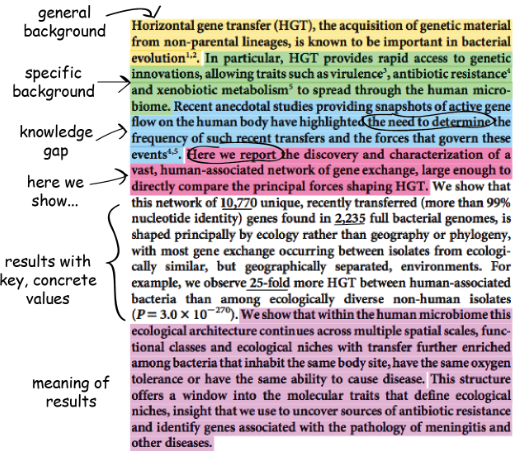
\includegraphics[scale=0.5]{image/good_abstract.png}
	\end{center}
	\caption{The Orion Nebula, M42, recorded with the CDK20N telescope on the night of November 1, 2011.}
	\label{fig:graph1}
\end{figure}

In text $e=mc^2$ and $\frac{1}{2n-1}$.\\

%------------------------------------------
%             tables
%------------------------------------------
\begin{equation}
\frac{x}{y}, \quad
\frac{\delta{f}}{\delta(x)},\quad
\frac{\partial^{2}{f}}{\partial{x}{^2}}
\end{equation}

   
%------------------------------------------
%             Tikz
%------------------------------------------
\begin{center}
%grid-2D-coordinates

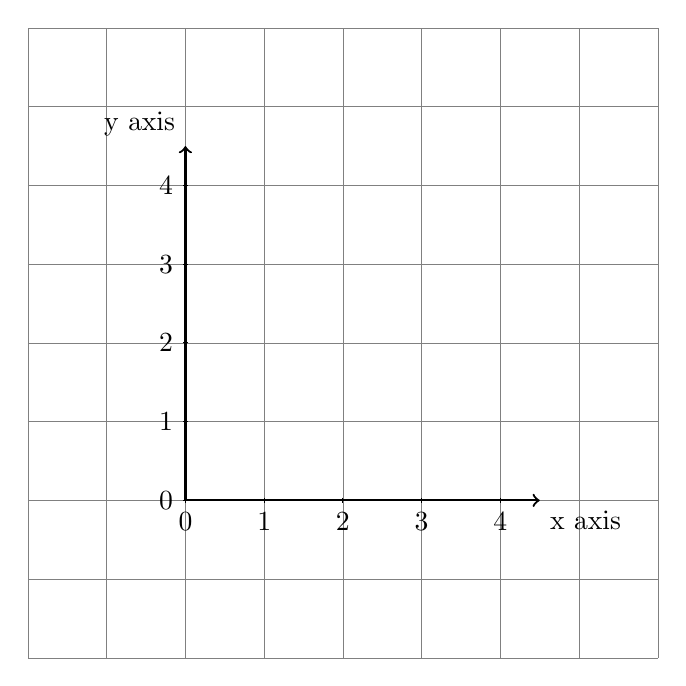
\begin{tikzpicture}
\draw[step=1cm,gray,very thin] (-2,-2) grid (6,6);
\draw[thick,->] (0,0) -- (4.5,0) node[anchor=north west] {x axis};
\draw[thick,->] (0,0) -- (0,4.5) node[anchor=south east] {y axis};

\foreach \x in {0,1,2,3,4}
   \draw (\x cm,1pt) -- (\x cm,-1pt) node[anchor=north] {$\x$};
\foreach \y in {0,1,2,3,4}
    \draw (1pt,\y cm) -- (-1pt,\y cm) node[anchor=east] {$\y$};

\end{tikzpicture}

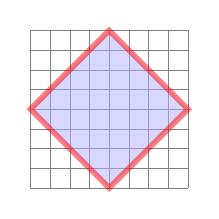
\begin{tikzpicture}
	\draw[step=0.25cm,gray,very thin] (-1,-1) grid (1,1);
	\draw[fill,color=blue!30,draw=red,line width=2pt, opacity=0.5] (1,0) -- (0,1) -- (-1,0) -- (0,-1) -- cycle;
\end{tikzpicture}

\begin{tikzpicture}
	\draw (0,0) grid(5,6);
	\draw (-2,8) rectangle(0,0);
	\draw (0,0) circle (2);
	\draw (5,5) circle (3 and 5);
	\draw (5,8) arc(-90:90:5);
\end{tikzpicture}


\end{center}

%rotation coordinate1
\tdplotsetmaincoords{60}{110}

\begin{tikzpicture}[scale=3,tdplot_main_coords]
\draw[thick,->] (0,0,0) -- (1,0,0) node[anchor=north east]{$x$};
\draw[thick,->] (0,0,0) -- (0,1,0) node[anchor=north west]{$y$};
\draw[thick,->] (0,0,0) -- (0,0,1) node[anchor=south]{$z$};
\coordinate (Shift) at (2,2,2);
\tdplotsetrotatedcoords{-20}{10}{0}
\tdplotsetrotatedcoordsorigin{(Shift)}
\draw[thick,color=blue,tdplot_rotated_coords,->] (0,0,0)
-- (1,0,0) node[anchor=south east]{$x'$};
\draw[thick,color=blue,tdplot_rotated_coords,->] (0,0,0)
-- (0,1,0) node[anchor=west]{$y'$};
\draw[thick,color=blue,tdplot_rotated_coords,->] (0,0,0)
-- (0,0,1) node[anchor=south]{$z'$};
\tdplotsetrotatedthetaplanecoords{30}
\draw[thick,color=blue,tdplot_rotated_coords,->] (0,0,0)
-- (.5,0,0) node[anchor=south east]{$x''$};
\draw[thick,color=blue,tdplot_rotated_coords,->] (0,0,0)
-- (0,.5,0) node[anchor=west]{$y''$};
\draw[thick,color=blue,tdplot_rotated_coords,->] (0,0,0)
-- (0,0,.5) node[anchor=south]{$z''$};
\end{tikzpicture}


%3D_rotation_coordinate
%start tikz picture, and use the tdplot_main_coords style to implement the display 
%coordinate transformation provided by 3dplot


\begin{tikzpicture}[scale=5,tdplot_main_coords]

%Angle Definitions
%-----------------

%set the plot display orientation
%synatax: \tdplotsetdisplay{\theta_d}{\phi_d}
\tdplotsetmaincoords{60}{110}

%define polar coordinates for some vector
%TODO: look into using 3d spherical coordinate system
\pgfmathsetmacro{\rvec}{.8}
\pgfmathsetmacro{\thetavec}{30}
\pgfmathsetmacro{\phivec}{60}
%set up some coordinates 
%-----------------------
\coordinate (O) at (0,0,0);

%determine a coordinate (P) using (r,\theta,\phi) coordinates.  This command
%also determines (Pxy), (Pxz), and (Pyz): the xy-, xz-, and yz-projections
%of the point (P).
%syntax: \tdplotsetcoord{Coordinate name without parentheses}{r}{\theta}{\phi}
\tdplotsetcoord{P}{\rvec}{\thetavec}{\phivec}

%draw figure contents
%--------------------

%draw the main coordinate system axes
\draw[thick,->] (0,0,0) -- (1,0,0) node[anchor=north east]{$x$};
\draw[thick,->] (0,0,0) -- (0,1,0) node[anchor=north west]{$y$};
\draw[thick,->] (0,0,0) -- (0,0,1) node[anchor=south]{$z$};

%draw a vector from origin to point (P) 
\draw[-stealth,color=red] (O) -- (P);

%draw projection on xy plane, and a connecting line
\draw[dashed, color=red] (O) -- (Pxy);
\draw[dashed, color=red] (P) -- (Pxy);

%draw the angle \phi, and label it
%syntax: \tdplotdrawarc[coordinate frame, draw options]{center point}{r}{angle}{label options}{label}
\tdplotdrawarc{(O)}{0.2}{0}{\phivec}{anchor=north}{$\phi$}


%set the rotated coordinate system so the x'-y' plane lies within the
%"theta plane" of the main coordinate system
%syntax: \tdplotsetthetaplanecoords{\phi}
\tdplotsetthetaplanecoords{\phivec}

%draw theta arc and label, using rotated coordinate system
\tdplotdrawarc[tdplot_rotated_coords]{(0,0,0)}{0.5}{0}{\thetavec}{anchor=south west}{$\theta$}

%draw some dashed arcs, demonstrating direct arc drawing
\draw[dashed,tdplot_rotated_coords] (\rvec,0,0) arc (0:90:\rvec);
\draw[dashed] (\rvec,0,0) arc (0:90:\rvec);

%set the rotated coordinate definition within display using a translation
%coordinate and Euler angles in the "z(\alpha)y(\beta)z(\gamma)" euler rotation convention
%syntax: \tdplotsetrotatedcoords{\alpha}{\beta}{\gamma}
\tdplotsetrotatedcoords{\phivec}{\thetavec}{0}

%translate the rotated coordinate system
%syntax: \tdplotsetrotatedcoordsorigin{point}
\tdplotsetrotatedcoordsorigin{(P)}

%use the tdplot_rotated_coords style to work in the rotated, translated coordinate frame
\draw[thick,tdplot_rotated_coords,->] (0,0,0) -- (.5,0,0) node[anchor=north west]{$x'$};
\draw[thick,tdplot_rotated_coords,->] (0,0,0) -- (0,.5,0) node[anchor=west]{$y'$};
\draw[thick,tdplot_rotated_coords,->] (0,0,0) -- (0,0,.5) node[anchor=south]{$z'$};

%WARNING:  coordinates defined by the \coordinate command (eg. (O), (P), etc.)
%cannot be used in rotated coordinate frames.  Use only literal coordinates.  

%draw some vector, and its projection, in the rotated coordinate frame
\draw[-stealth,color=blue,tdplot_rotated_coords] (0,0,0) -- (.2,.2,.2);
\draw[dashed,color=blue,tdplot_rotated_coords] (0,0,0) -- (.2,.2,0);
\draw[dashed,color=blue,tdplot_rotated_coords] (.2,.2,0) -- (.2,.2,.2);

%show its phi arc and label
\tdplotdrawarc[tdplot_rotated_coords,color=blue]{(0,0,0)}{0.2}{0}{45}{anchor=north west,color=black}{$\phi'$}

%change the rotated coordinate frame so that it lies in its theta plane.
%Note that this overwrites the original rotated coordinate frame
%syntax: \tdplotsetrotatedthetaplanecoords{\phi'}
\tdplotsetrotatedthetaplanecoords{45}

%draw theta arc and label
\tdplotdrawarc[tdplot_rotated_coords,color=blue]{(0,0,0)}{0.2}{0}{55}{anchor=south west,color=black}{$\theta'$}

\end{tikzpicture}


\newpage
\begin{center}
\begin{figure}
\subfigure[abc]{
%rotation coordinate1
\tdplotsetmaincoords{60}{110}

\begin{tikzpicture}[scale=3,tdplot_main_coords]
\draw[thick,->] (0,0,0) -- (1,0,0) node[anchor=north east]{$x$};
\draw[thick,->] (0,0,0) -- (0,1,0) node[anchor=north west]{$y$};
\draw[thick,->] (0,0,0) -- (0,0,1) node[anchor=south]{$z$};
\coordinate (Shift) at (2,2,2);
\tdplotsetrotatedcoords{-20}{10}{0}
\tdplotsetrotatedcoordsorigin{(Shift)}
\draw[thick,color=blue,tdplot_rotated_coords,->] (0,0,0)
-- (1,0,0) node[anchor=south east]{$x'$};
\draw[thick,color=blue,tdplot_rotated_coords,->] (0,0,0)
-- (0,1,0) node[anchor=west]{$y'$};
\draw[thick,color=blue,tdplot_rotated_coords,->] (0,0,0)
-- (0,0,1) node[anchor=south]{$z'$};
\tdplotsetrotatedthetaplanecoords{30}
\draw[thick,color=blue,tdplot_rotated_coords,->] (0,0,0)
-- (.5,0,0) node[anchor=south east]{$x''$};
\draw[thick,color=blue,tdplot_rotated_coords,->] (0,0,0)
-- (0,.5,0) node[anchor=west]{$y''$};
\draw[thick,color=blue,tdplot_rotated_coords,->] (0,0,0)
-- (0,0,.5) node[anchor=south]{$z''$};
\end{tikzpicture}


}
\hfill
\subfigure[abc]{
%3D_rotation_coordinate
%start tikz picture, and use the tdplot_main_coords style to implement the display 
%coordinate transformation provided by 3dplot


\begin{tikzpicture}[scale=5,tdplot_main_coords]

%Angle Definitions
%-----------------

%set the plot display orientation
%synatax: \tdplotsetdisplay{\theta_d}{\phi_d}
\tdplotsetmaincoords{60}{110}

%define polar coordinates for some vector
%TODO: look into using 3d spherical coordinate system
\pgfmathsetmacro{\rvec}{.8}
\pgfmathsetmacro{\thetavec}{30}
\pgfmathsetmacro{\phivec}{60}
%set up some coordinates 
%-----------------------
\coordinate (O) at (0,0,0);

%determine a coordinate (P) using (r,\theta,\phi) coordinates.  This command
%also determines (Pxy), (Pxz), and (Pyz): the xy-, xz-, and yz-projections
%of the point (P).
%syntax: \tdplotsetcoord{Coordinate name without parentheses}{r}{\theta}{\phi}
\tdplotsetcoord{P}{\rvec}{\thetavec}{\phivec}

%draw figure contents
%--------------------

%draw the main coordinate system axes
\draw[thick,->] (0,0,0) -- (1,0,0) node[anchor=north east]{$x$};
\draw[thick,->] (0,0,0) -- (0,1,0) node[anchor=north west]{$y$};
\draw[thick,->] (0,0,0) -- (0,0,1) node[anchor=south]{$z$};

%draw a vector from origin to point (P) 
\draw[-stealth,color=red] (O) -- (P);

%draw projection on xy plane, and a connecting line
\draw[dashed, color=red] (O) -- (Pxy);
\draw[dashed, color=red] (P) -- (Pxy);

%draw the angle \phi, and label it
%syntax: \tdplotdrawarc[coordinate frame, draw options]{center point}{r}{angle}{label options}{label}
\tdplotdrawarc{(O)}{0.2}{0}{\phivec}{anchor=north}{$\phi$}


%set the rotated coordinate system so the x'-y' plane lies within the
%"theta plane" of the main coordinate system
%syntax: \tdplotsetthetaplanecoords{\phi}
\tdplotsetthetaplanecoords{\phivec}

%draw theta arc and label, using rotated coordinate system
\tdplotdrawarc[tdplot_rotated_coords]{(0,0,0)}{0.5}{0}{\thetavec}{anchor=south west}{$\theta$}

%draw some dashed arcs, demonstrating direct arc drawing
\draw[dashed,tdplot_rotated_coords] (\rvec,0,0) arc (0:90:\rvec);
\draw[dashed] (\rvec,0,0) arc (0:90:\rvec);

%set the rotated coordinate definition within display using a translation
%coordinate and Euler angles in the "z(\alpha)y(\beta)z(\gamma)" euler rotation convention
%syntax: \tdplotsetrotatedcoords{\alpha}{\beta}{\gamma}
\tdplotsetrotatedcoords{\phivec}{\thetavec}{0}

%translate the rotated coordinate system
%syntax: \tdplotsetrotatedcoordsorigin{point}
\tdplotsetrotatedcoordsorigin{(P)}

%use the tdplot_rotated_coords style to work in the rotated, translated coordinate frame
\draw[thick,tdplot_rotated_coords,->] (0,0,0) -- (.5,0,0) node[anchor=north west]{$x'$};
\draw[thick,tdplot_rotated_coords,->] (0,0,0) -- (0,.5,0) node[anchor=west]{$y'$};
\draw[thick,tdplot_rotated_coords,->] (0,0,0) -- (0,0,.5) node[anchor=south]{$z'$};

%WARNING:  coordinates defined by the \coordinate command (eg. (O), (P), etc.)
%cannot be used in rotated coordinate frames.  Use only literal coordinates.  

%draw some vector, and its projection, in the rotated coordinate frame
\draw[-stealth,color=blue,tdplot_rotated_coords] (0,0,0) -- (.2,.2,.2);
\draw[dashed,color=blue,tdplot_rotated_coords] (0,0,0) -- (.2,.2,0);
\draw[dashed,color=blue,tdplot_rotated_coords] (.2,.2,0) -- (.2,.2,.2);

%show its phi arc and label
\tdplotdrawarc[tdplot_rotated_coords,color=blue]{(0,0,0)}{0.2}{0}{45}{anchor=north west,color=black}{$\phi'$}

%change the rotated coordinate frame so that it lies in its theta plane.
%Note that this overwrites the original rotated coordinate frame
%syntax: \tdplotsetrotatedthetaplanecoords{\phi'}
\tdplotsetrotatedthetaplanecoords{45}

%draw theta arc and label
\tdplotdrawarc[tdplot_rotated_coords,color=blue]{(0,0,0)}{0.2}{0}{55}{anchor=south west,color=black}{$\theta'$}

\end{tikzpicture}

}
\end{figure}
\end{center}

%------------------------------------------
%             Objectives
%------------------------------------------
\subsection*{How to write Objectives}
"Provide a clearly defined statement of the objectives of the research." Sometimes only one objective; sometimes one board AIM, and several objectives.\\
Use active verbs, i.e. propose, create, construct, demonstrate, define, establish, differentiate.
\begin{enumerate}[(i)]
  \item The labels consists of sequential numbers.  
  \begin{itemize}
  	\item The individual entries are indicated with a black dot, a so-called bullet.
  	\item The text in the entries may be of any length.
  \end{itemize}
  \item The numbers starts at 1 with every call to the enumerate environment.
\end{enumerate}
%-------------------------------------------------------
%				Dexterous Motion Planning
%-------------------------------------------------------
\noindent\uline{Dexterous motion planning.} The robot dexterous ma


While Okamura \cite{Okamura_2000_Overview_DM} divided dexterous motion planning into two main categories including the motion planning of the object to acquire a desired configuration and the grasp planning in terms of contact forces optimization.\\

\cite{Trinkle90_Planning_DexManipulation, Trinkle_1991_framework_Planning_DM, Munoz95_Dex.Manipulation_Geo}\\

The article \cite{Bicchi_2000_Hands_Dexterous} focused on three main categories namely manipulative dexterity, grasp robustness, and human operability.
\begin{enumerate}
    \item{Manipulative dexterity: the capability of the hand to manipulate objects so as to relocate them arbitrarily for the purposes of the tasks.}
    \item{Grasp robustness is the capability of keeping hold of manipulated objects in spite of all possible disturbances (unexpected forces, erroneous estimates of the object characteristics, etc.) while maintaining a "gentle” enough grip not to cause any damage.}
	\item{Human operability: the allowance for an easy and friendly interface with the human operator.}
\end{enumerate}
%------------------------------------------
%             Dr. Lei Research Proposal
%------------------------------------------
\newpage
\subsection{Dr. Lei Research Proposal}
\subparagraph{1-Aim}
\textcolor{red}{To develop a discrete rolling contact theory for tactile fingertips.}\\

\noindent\uline{Lack of discrete contact theory for tactile fingertips.} Tactile fingertips have been increasingly used in robot hands in recent years to enhance their dexterity and adaptability. The geometric differential properties of the discretised fingertip surfaces need to be approximated to be used. In this respect, tools such as the \textbf{moving frame} and \textbf{curvatures in discrete differential geometry} provide a consistent and computationally efficient method to approximate these entities. However, \textcolor{red}{\textbf{these tools have not been applied to in-hand manipulation}.}\\


\noindent\uline{Novelty and Impact.} This project will also employ the \emph{tools} developed in \emph{discrete differential geometry} \textbf{to establish \textcolor{red}{a discrete contact theory} of discrete surfaces}, which will be integrated into the proposed pure geometric framework. This project will eradicate the barriers that have hindered the progress of in-hand manipulation and enable robot hands to be used in advanced manufacturing and ultimately to have dexterity and adaptability comparable to the human hand.\\

\subparagraph{2-Background}
\begin{itemize}
\item Rolling contact in human in-hand manipulation
\item Rolling contact in robot hands
\item Vectorial kinematics of multifingered hands
\item Lie group and Lie algebra in kinematics multifingered hands
\item Contact theory via Cantan’s moving frame method
\item Singularity theory for in-hand manipulation
\item \textbf{Discrete contact theory for tactile fingertips}. In recent years, tactile sensors have been added to fingertips of robot hands to emulate human sensing in grasping and manipulation \cite{Lei-Bagnell12_Tactile_Autonomous, HaoDang11_Tactile_BlindGrasping, Rothling07_Dex.Manipulators_Tactile, Zhang14_Tactile_DynamicGrasping}. These grid-based tactile sensors naturally discretise the surfaces of fingertips into \emph{quadrilateral faces}, where the discrete equivalents of notions and methods in differential geometry, such as \textbf{curvatures and the moving frame method}, can be extended \cite{Bobenko10_Discrete_Curvature, Sullivan08_Curvature_DiscreteSurface}. 

Recent progress in discrete differential geometry introduces tools to \textbf{approximate geometric attributes}, especially \textbf{the moving frames and curvatures}, which are guaranteed \emph{to be appropriate extension from the continuous to the discrete setting} \cite{Meyer03_Discrete_Diff.Geo_2Manifolds, Xu13_Geo.Diff_Discrete, Hameiri03_Darboux_Curvature_Discrete}. However, \textcolor{red}{these new tools have not been applied to in-hand manipulation}.
\end{itemize}



\begin{itemize}
\item [25] H. Dang, J. Weisz, and P. K. Allen, "Blind grasping: Stable robotic grasping using tactile feedback and hand kinematics,"
\item [26] F. Röthling."Platform portable anthropomorphic grasping with the bielefeld 20-dof shadow and 9-dof tum hand," 
\item [27] T. Zhang. "Multifingered robot hand dynamic grasping control based on fingertip three-axis tactile sensor feedback," 
\item [28] A. I. Bobenko."A curvature theory for discrete surfaces based on mesh parallelity,"
\item [29] J. M. Sullivan, "Curvatures of smooth and discrete surfaces," in Discrete differential geometry
\item [30] M. Meyer,"Discrete differential-geometry operators for triangulated 2-manifolds," 
\item [31] G. Xu, "Consistent approximations of several geometric differential operators and their convergence,"
\item [32] E. Hameiri. "Estimating the principal curvatures and the Darboux frame from real 3-D range data,"
\end{itemize}

\subparagraph*{3-Significance} \mbox{}\\

\uline{\textcolor{red}{A new discrete rolling contact theory.}} The moving frame method and curvature theory in differential geometry have their counterparts in discrete differential geometry. \textcolor{blue}{An ever increasing number of robot fingertips are equipped with tactile sensors, and these grid-based sensors naturally mesh the fingertips into discrete surfaces} \cite{Lei14_Teleoperation_ThumbRobotHand,  Bagnell12_IntegratedSystem_AutonomousRoboticsManipulation}.
As I pioneered applying \textcolor{blue}{the curvature theory in differential geometry to in-hand manipulation} \cite{Lei09_coordinate-free_instantaneous_kinematics, Lei10_Darboux-Frame, Lei10_Geometric.Kinematics_PointContact, Lei15_PolynomialFormulation_InverseKinematics, Lei15_sliding.rolling.loci_kinematics, Lei09_Kinematic.Geometry_Circular.Surfaces}, I will initiate applying \textcolor{red}{the discrete} \textcolor{blue}{curvature theory} to in-hand manipulation. I will exploit the rich toolset developed in the communities of discrete differential geometry and computer graphics. I will develop a new discrete contact theory
and integrate it into the proposed geometric framework.

\newpage

\cite{Belta_2005_Discrete_MP} (Discrete abstractions for robot motion planning and control in polygonal environments)
\subparagraph{4-Research Design and Method}
\subparagraph*{Overview} Further, I will develop a new discrete contact theory by extending my pioneering work and applying the recent progress in discrete differential geometry.\\

\textbf{Aim 2}: \textbf{To develop a discrete contact theory.}\\

\uline{\textbf{Rationale}}. The grid-based tactile sensors naturally discretise the fingertip surfaces into quadrilateral faces, which can be converted into triangle meshes that have been extensively used in Computer Graphics \cite{Martin04_Quadrilateral_Discrete}. Contact theory requires an approximation of the first and second order properties, such as curvatures and principle directions \cite{Lei10_Darboux-Frame, Montana88_Kinematics_Contact_Grasp}. The current patch-based contact theory needs analytical evaluation, which often introduces overshooting or unexpected surface behaviour. 

On the other hand, moving frame and curvatures can be consistently derived by the rich tool set developed in discrete differential geometry, and these appropriations are guaranteed to be an extension from the continuous to the discrete setting \cite{Meyer03_Discrete_Diff.Geo_2Manifolds}.\\

\uline{\textbf{Theoretical approach}.} I propose to apply \emph{the tool set} developed in \textbf{discrete differential geometry to establish a discrete contact theory}. My contact theory for smooth surfaces is formulated in terms of the moving frame, normal curvature, geodesic curvature, and geodesic torsion [\cite{Lei09_coordinate-free_instantaneous_kinematics, Lei10_Darboux-Frame, Lei15_PolynomialFormulation_InverseKinematics, Lei15_sliding.rolling.loci_kinematics, Lei10_PhDThesis}. \emph{Each of these geometric entities has its counterpart in discrete differential geometry}, as in Fig. 5 (Lei's PhD thesis \cite{Lei10_PhDThesis}). When I was deriving the contact theory, the velocity constraint was embedded in the arc length, \textcolor{red}{eliminating the need of nonlinear differential equations} and \textcolor{blue}{facilitating grid-based path planning}, as in Fig. 6 (in \cite{Lei09_coordinate-free_instantaneous_kinematics}). I \emph{will apply the same approach} in the \emph{discrete case} \textbf{to establish a discrete contact theory} that is coordinate-independent and does not involve difference terms.\\


\uline{\textbf{Empirical validation}.} The BarrettHand is equipped with tactile sensors capable of providing 96 cells of tactile-array data spread across all three fingers and the palm. The density of cells becomes higher towards the very tips of the fingers where finer spatial resolution is desirable \cite{Martin04_Quadrilateral_Discrete}. The embedded signal processing of raw data from the tactile sensors can determine point of contact, and this will facilitate validation of the proposed discrete contact theory.

\subparagraph{Reference}
\begin{itemize}
\item 1 From Dr.LeiCui research : \cite{Lei10_Darboux-Frame, Lei10_Geometric.Kinematics_PointContact, Lei11_Posture.Workspace_Multifinger, Lei12_Polynomial_Inverse.Kinematics, Lei12_ReciprocityBased_SVD_Inverse.Kinematics, Lei15_sliding.rolling.loci_kinematics, Lei15_PolynomialFormulation_InverseKinematics, Lei18_Rolling.Contact_Kinematics_Multifinger, Lei17_In-Hand_Forward.Inverse.Kinematics, Lei07_Euclidean_Invariants, Lei09_Kinematic.Geometry_Circular.Surfaces, Lei09_Orientation-Workspace_Metahand, Lei09_coordinate-free_instantaneous_kinematics}
\item 2 Text book about dynamic-discrete \cite{Book_Rosenberg77_DynamicsDiscrete}
\end{itemize}


%==============================================================
\subsection{Markov Decision Process}
\noindent\uline{Introduction.} 
Markov Decision Process (MDP) is an extension of a Markov chain which is a stochastic model in discrete time. MDP represents a mathematical framework to model decision making process that has been studied in early \cite{Howard60_DP_MDP, Miller68_MDP}. For the record, many applied study may have an implicit underlying the MDP framework to determine the expected cost of raw material that the stock can purchase or shortage \cite{White85_ApplicationMDP}, to control the pest or protect natural resources \cite{White93_ApplicationMDP}. In the robotic field, the MDP has been successfully applied for path planning problems such as combination with a quadtree decomposition of the environment to compute the motion plan \cite{Burlet04_MP_MDP} or association with ideas of deterministic search and dynamic programming techniques to reduce the processing cost and improve performance path planning algorithm \cite{Ferguson04_MDP_Pathplanning}. Another promising technique for autonomous trajectory planning is based on the MDP with clothoid tentacles \cite{Muhager16_MDP_Clothes}. The study used stochastic transitions \cite{Puterman14_Book_MDP_DiscreteDP} that can reduce the presence of distant obstacles in an occupancy grid.\\


%==============================================================
\noindent\uline{The agent-environment interface.} 
As shown in Figure \ref{fig:MDP1}, there are two main objects in the MDP including an agent and the environment that they interact together at each of a sequence of discrete time steps, $t=0,1,2,3,...$. The process in some states $S_t$ at each time step $t$ is described that the decision maker chooses any action $A_t$ in the state and the agent will receive the reward $R_t$ from the environment. In \cite{SuttonBarto18_RLbook}, the general rule of agent-environment boundary is not the same as the physical boundary of a robot's or animal's body. In some cases, the agent may know everything in the environment, just as the rewards which are computed from the agent's action function or the state received. However, in another case of solving puzzle like Rubik's cube, the agent knows all the environment such as colors, faces and dimensions but hard to solve its work.
\begin{figure}[h]
	\begin{center}
	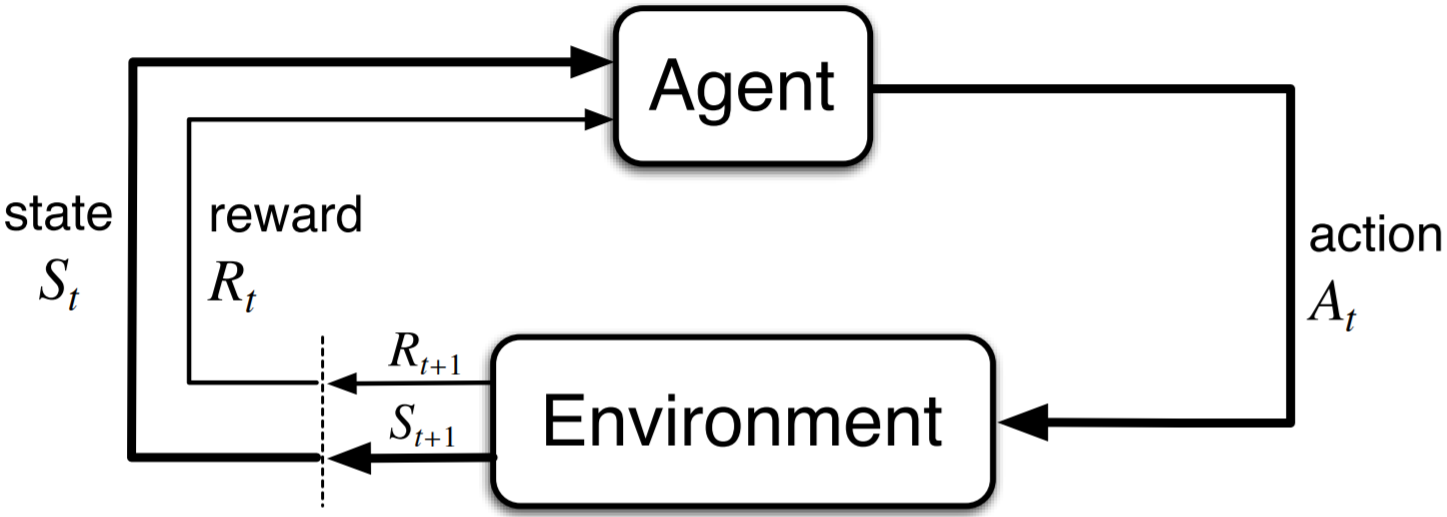
\includegraphics[width=0.5\textwidth]{image/SuttonBartoI_RL.png}
	%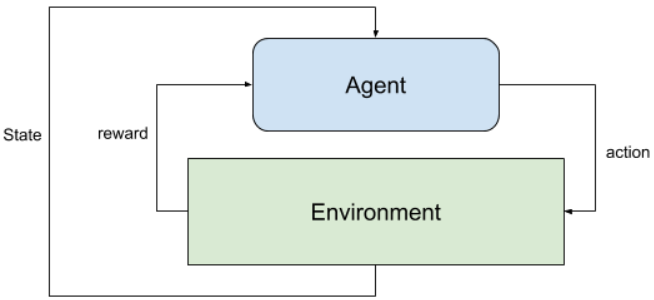
\includegraphics[scale=0.5]{image/MDP.png}
	\end{center}
	\caption{The interaction of agent and environment \cite{SuttonBarto18_RLbook}.}
	\label{fig:MDP1}
\end{figure}


%==============================================================
\noindent MDP is a tuple $<S,A,T,r,\gamma>$ where $S$ is a set of observations when the agent observes a state from the environment; $S$ is a set of actions that the agent can execute from the task to interact with the environment; $T$ is transition probability matrix in which of making the action $a \in A$ from the current state $s \in S$ to the next state $s'$ ($T(s'|s,a)=\mathbb{P}[S_t=s, A_t=a]$); $r$ is the reward model that the agent can receive in the state $s$ when executing an action $a$ ($r(s,a)=\mathbb{E}[R_{t+1}|S_t=s, A_t=a]$), and $\gamma$ is the discount factor where $0<\gamma<1$ that relatives between immediate and future rewards. In path planning problems, the MDP method is applied for finding the path in terms of optimizing the expected sum of discounted rewards and the Bellman equation \cite{Bellman57_MDP} can be promoted in the study.\\ 

%==============================================================
%\noindent\uline{Reinforcement learning.} RL is one part of machine learning which does not require the environment model or the dynamic system as well. \\


%==============================================================
\noindent\uline{Bellman equation.} Before discussing the Bellman equation, there are some of principal components of the Reinforcement Learning framework including Reward and Return, Policies, and Value functions which are briefly introduced as following. \\
\noindent In reinforcement learning, there are two types of value function used to optimize the policy including the state value function $
V^{\pi}(s)=\mathbb{E}_{\pi}[R_t|s_t=s]
$ and the action value function $
Q^{\pi}(s,a)=\mathbb{E}_{\pi}[s_t=s,a_t=a]
$. They are the expected returns generated from the state and action under the policy $\pi$.
The value function changes dependently on the policy for the same environment due to that fact that the value of the state changes dependently and expected rewards will be received. The action value function represents the value of taking an action in some state $s$.\\

\noindent If we call $\mathcal{P}$ is the transition probability from starting state $s$, taking action $a$, then ending up in state $s'$, we have 
$
\mathcal{P}^a_{ss'}=pr(s_{t+1}=s'|s_t=s,a_t=a)
$. 
In addition, $\mathcal{R}^a_{ss'}$ is called the expected reward received from starting state $s$, taking action $a$, and moving into state $s'$, we have 
$
\mathcal{R}^a_{ss'}=\mathbb{E}[r_{t+1}|s_t=s,s_{t+1}=s',a_t=a]
$

\noindent Finally, the Bellman equation \cite{Bellman57_MDP} can be derived for the on-policy state value function with the results is as follows:
\begin{equation}
V^{\pi}(s) = \sum_{a}\pi(s,a)\sum_{s'}\mathcal{P}^a_{ss'}[\mathcal{R}^a_{ss'}+\gamma{V}^{\pi}(s')]
\end{equation}
and for the on-policy action value function as:
\begin{equation}
Q^{\pi}(s,a) = \sum_{s'}\mathcal{P}^a_{ss'}[\mathcal{R}^a_{ss'}+\gamma\sum_{a'}\pi(s',a'){Q}^{\pi}(s',a')]
\end{equation}
for all $s\in{S}, a\in{A(s)}$.

\noindent It is noticed that the Bellman equation can represent the values of states as values of other states like easily calculating the value of state $s_t$ when knowing the value of state $s_{t+1}$. However, to apply for the stochastic shortest path problems by using the Bellman equation, there are techniques such as  value iteration, policy iteration, and linear programming should be taken into consideration to solve the Bellman equation. \\

%==============================================================
\noindent\uline{Value iteration.} This is one of the method to find an optimal policy is to determine the optimal value function. The method in detail to converge to the correct $V^*$ values that can be performed by an iterative algorithm \cite{Bellman57_DynamicProgramming, Bertsekas87_DynamicProgramming}. The Bellman equation for the optimal value function is as follows:
\begin{equation}
Q^{*}(s,a) 
= \mathbb{E}[R_{t+1} + \gamma \max_{a'}Q^{*}(S_{t+1},a')|S_{t}=s, A_{t}=a] 
= \sum_{s',r}p(s',r|s,a)[r+\gamma \max_{a'}Q^{*}(s',a')] 
\end{equation}
The algorithm will stop when the value function changes in a small amount of one update of each state (sweep). The combination of one sweep of policy evaluation and one sweep of policy improvement in the value iteration algorithm can make the convergence faster. It is also noted that the value iteration can be obtained when the step of updating the Bellman optimality equation happens and the updated value has to be required maximum over all actions. \\

%==============================================================
\noindent\uline{Policy iteration.} Policy iteration algorithm can be defined as another way of determining an optimal policy in a finite number iteration. The iteration starts with the value function $V(s)$ of the previous policy $\pi$ in each policy iteration as $\pi_0\xrightarrow{E}v_{\pi_0}\xrightarrow{I}\pi_1\xrightarrow{E}v_{\pi_1}\xrightarrow{I}\pi_2\xrightarrow{E} ... {\pi_*}\xrightarrow{E}v_*$, where $\xrightarrow{E}$ denotes a policy evaluation and $\xrightarrow{I}$ indicates a policy improvement. The Bellman equation for the optimal value function as the policy iteration is:
\begin{equation}
V^{*}(s) 
= \max_{a} \mathbb{E}[R_{t+1} + \gamma V^{*}(S_{t+1})|S_{t}=s, A_{t}=a] = \max_{a} \sum_{s',r}p(s',r|s,a)[r+\gamma V^{*}(s')]
\end{equation}
The policy iteration algorithm may converge only few iterations that will be gained the expected infinite discounted reward by executing the policy \cite{SuttonBarto18_RLbook}: 
\begin{equation}
\pi'(s)=argmax_{a}(R(s,a)+\gamma \sum_{s'\in S} p(s',r|s,a)V^{\pi}(s'))
\end{equation}

%==============================================================
\noindent\uline{Linear programming.} Linear programming methods can be used to solve the Bellman equation and they are better than dynamic programming in some cases as less number of states and a potential method in the curse of dimensionality.
The significant application of the linear programming based path planning algorithm is to derive optimal paths for robotics in various kinds of environment \cite{Chasparis05_PP_LinearProgramming}. The article proposed a linear formulation for resource allocation of the path planning issue. Integrating linear programming to a receding horizon implementation for multi-vehicle path planning is introduced as a model simplification. To describe the feasible path planning, the paper also used stochastic models which can propose the current position and predict the future trajectories. Another implementation of linear programming from \cite{Yang12_PP_LinearProgramming} for the path planning problems has been focus on obstacle avoidance. The most advantage of this improvement is to reduce the computation time cost in the real time computation for the path planning process.

\section{Table Notes}


\begin{table}[ht]
\centering
\caption{Thicker horizontal lines above and below the table.}
\begin{tabular}{lcc}
\toprule
&Treatment A&Treatment B\\ 
\hline
%\midrule
John Smith&1&2\\
Jane Doe&--&3\\
Mary Johnson&4&5\\
\bottomrule
\end{tabular}
\end{table}%


Sometimes very long tables must be presented which may also go over pages. \\


\begin{table}[ht!]
     \centering
     \caption{Caption text} 
     \begin{tabular}{|p{5cm}|p{5cm}|}
        \toprule 	
	\bfseries{Resources} &\bfseries{Provider}\\ \hline
	Robot Operating Software & Open Source\\
	MatLab                  & Curtin University\\
	ABB Robotic Arm         & Curtin University\\
	Computer and Printing   & Curtin University\\
	\bottomrule
      \end{tabular}
    \end{table}
    
\begin{table}[h]
 \centering
     \caption{Long table} 
\begin{tabularx}{\textwidth}{X|l}
  \textbf{Symptom} & \textbf{Metric} \\
\hline
Class that & ATFD is more than a few\\
Class that & WMC is high\\
Class that & TCC is low\\
\end{tabularx}
\end{table}


\begin{table}[ht]
\caption{Repetition of custom-defined column type.}
\begin{center}
\begin{tabular}{*{3}{V}}
\hline
aaa&bbb&ccc\\
\hline
aaa&bbb&ccc\\
aaa&bbb&ccc\\
\hline
\end{tabular}
\end{center}
\end{table}


%%\newpage
%%\textcolor{red}{•	Include a discussion of the motivation and advantages for rolling contact for in-hand manipulation\\
%%•	Reduce the length of the discussion on modelling the kinematics of rolling motion\\
%%•	Add a brief review of path planning for two general objects under nonholonomic constraints\\
%%•	Simply the aims: remove specific techniques and algorithms, and describe the broad aim of the project general terms, and in one or two sentences. Ensure that specific objectives are framed so that the aim can be achieved.\\
%%•	Include a section which describes how a discretised model will be produced such that the discrete planning algorithms described can be applied. How is this discrete model to be obtained from the continuous-time models discussed?\\
%%•	If optimal planning is discussed, ensure you are specific about in what sense the solution is optimal. In some cases, optimality is not required, only a satisfactory or satisficing solution in the sense of a cost function being below some bound. In such cases, sampling-based solutions (such as RRT) are appropriate.\\
%%•	Please also review the writing for grammatical correctness (seek some assistance on this if needed).\\
%%•	Note Robot Operating System (not Software) in Table 1.}\\
%
%%%==============================
%%%			%references
%%%==============================
%\cleardoublepage
%\bibliographystyle{ieeetr} %
%
%%\bibliographystyle{plain} % only number
%%\bibliographystyle{plainnat} % Author-year
%%\bibliographystyle{unsrtnat} %sort in number
%%\bibliography{refers, RC_RollingBall, RC_LeiCui, RC_basemanipulation, RC_MotionPlanning, RC_Bicchi, RC_Kinematics, Kinematics, DiscreteKinematics, InHandManipulation, tactile, disdiffgeo}
%
%\bibliography{citation}
%\addcontentsline{toc}{section}{\numberline{}{REFERENCES}}
%
%%%=============================={}
%%%			%Appendix
%%%==============================
\cleardoublepage
\appendix
\section{APPENDIX}
\label{appendix:A}
%
%\centering
%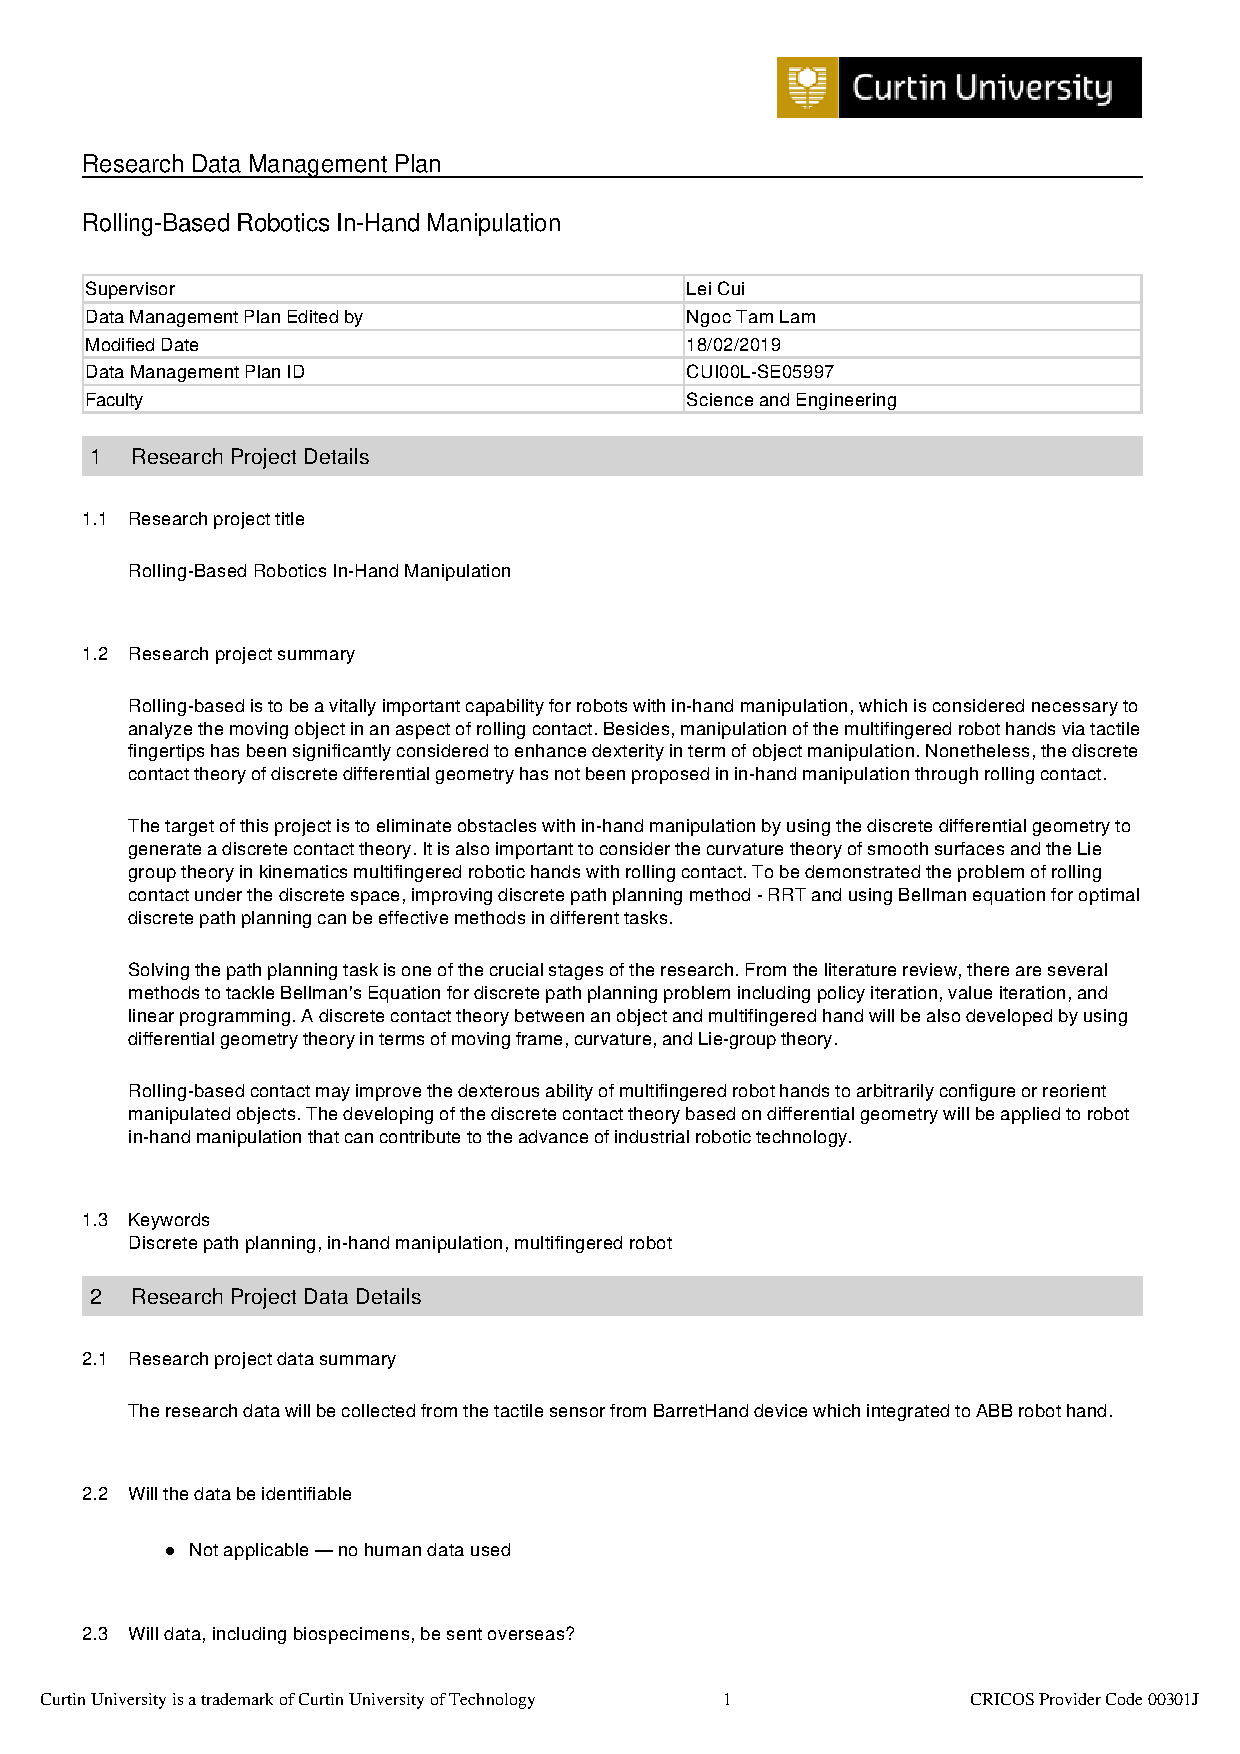
\includegraphics[scale=0.8]{DataManagement.pdf}
%
%\includepdf[pages=2]{DataManagement.pdf}

\printbibliography
\end{document}